\documentclass[a4paper,12pt]{article}

\usepackage{cmap}                   % поиск в PDF
\usepackage[T2A]{fontenc}           % кодировка
\usepackage[utf8]{inputenc}         % кодировка исходного текста
\usepackage[english,russian]{babel} % локализация и переносы
\usepackage{graphicx} % картинки

\author{Канушин Максим}
\title{Анализ разработанных задач в системе автоматической проверки для MOOC "Программирование модулей ядра Linux"}
\date{\today}

\begin{document} % Конец преамбулы, начало текста.

\maketitle
\section{Аннотация}
В данной работе исследуется статистика прохождения студентами массового открытого онлайн курса <<Программирование модулей ядра Linux>>. Проверка заданий, присланных студентами проходит в автоматическом режиме разработанной ранее системой. Задания представляют собой лабораторные работы, в рамках которых студенту необходимо разработать программу на языке С и Makefile. Целью исследования является определить насколько хорошо разработанные задачи и система их проверки соответствуют видео-лекциям.

\section{Введение}

\section{Описание проверяющей системы}
\subsection{Характеристики системы}
Система автоматической проверки лабораторных работ представляет из себя комплекс взаимосвязанных программных средств, позволяющих студенту загрузить разработанную им программу и получить ответ о ее корректности, а так же логи сборки, запуска и информацию о произошедших ошибках при их наличии.

Система обеспечивает:
\begin{itemize}
	\item Получение решения от студента
	\item Проверку корректности формата решения
	\item Сборку решения
	\item Запуск решения
	\item Проверку работы решения
	\item Отправку результатов решения обратно студенту
\end{itemize}

Система обеспечивает изолированность проверяемого решения от внешней среды, чтобы обеспечить достаточный уровень надежности и безопасности исполнения. Помимо этого исключается взаимное влияние решений друг на друга для того, чтобы не дать возможность студенту случайно или намеренно повлиять на работу другого студента или просмотреть его. Среда, в которой происходит проверка, одинакова для всех решений, чтобы обеспечить как одинаковые условия проверки различных решений, так и многократную воспроизводимость результатов проверки одного и того же решения.

\subsection{Архитектура системы}
Система состоит из двух связанных компонент: веб-приложения и демона.

Алгоритм работы системы состоит из нескольких этапов. При получении решения, веб-приложение сохраняет его в локальное хранилище на сервере. Демон, обнаружив, что в локальной директории появилось новое решение, в зависимости от задания выбирает соответствующий сценарий проверки и запускает виртуальную машину, на которой запускается набор скриптов, собирающих и запускающих решение, а так же проверяющего его. После окончания проверки, результаты, включая логи сборки и исполнения, выгружаются из виртуальной машины, после чего она выключается.

Полная схема проверяющей системы представлена на рис. 1.

\begin{figure}[h]
	\centering
	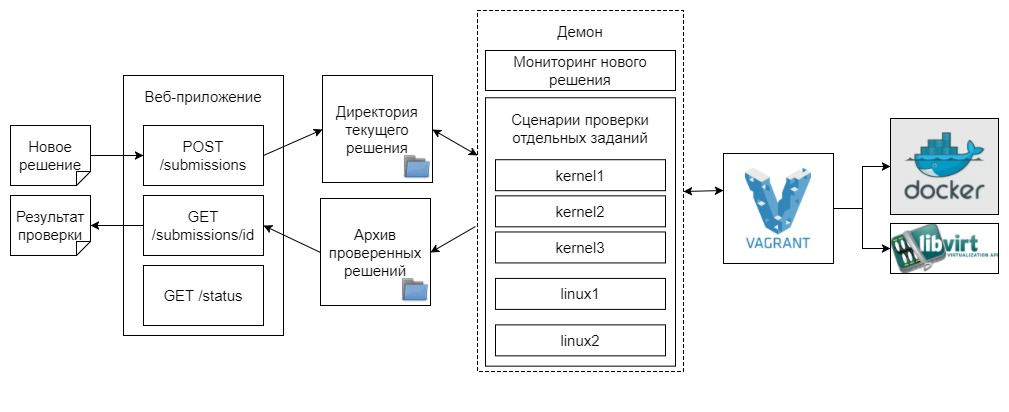
\includegraphics[width=\textwidth]{arch.jpg}
	\caption{Архитектура системы}
	\label{fig:mesh1}
\end{figure}

\section{Обзор результатов прохождения онлайн-курса}
Онлайн курс <<Программирование модулей ядра Linux>> был запущен в тестовом режиме. Курс состоял из 9 практических задач. В сумме по всем задачам было получено 795 решений из которых 270 правильных.

\subsection{Stopout}
Stopout - величина, показывающая, сколько человек прекратили прохождение курса на той или иной задаче. На рис. \ref{fig:mesh2} представлен график, показывающий распределение студентов, бросивших курс, по задачам до которых они добрались.

\begin{figure}[h]
 	\centering
	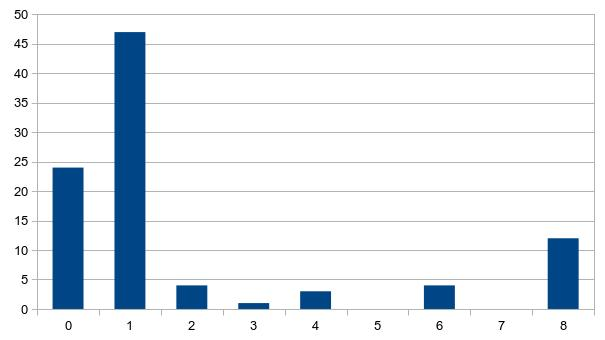
\includegraphics[width=\textwidth]{stopout.jpg}
	\caption{Stopout}
	\label{fig:mesh2}
\end{figure}

Первые два задания являются довольно простыми и схожими по сложности, что объясняет, почему многие студенты, выполнившие первое задание, решили и второе.

Данный критерий был посчитан для сравнения с исследованием из статьи \textit{Likely to stop? Predicting Stopout in Massive Open Online Courses} \cite{likelytostop}. На рис \ref{fig:mesh3} представлены его результаты на значительно более объемной выборке (154 тыс. студентов, 17.8 млн загруженных решений).

\begin{figure}[h]
	\centering
	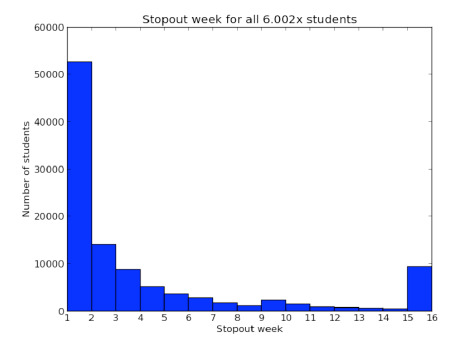
\includegraphics[width=\textwidth]{stopout_mit.jpg}
	\caption{Predicting Stopout in Massive Open Online Courses}
	\label{fig:mesh3}
\end{figure}
\pagebreak

\subsection{Пройденные студентами этапы в рамках задач}
По результатам проверки решений были подсчитаны этапы в рамках каждой задачи, которые удалось пройти студенту.

\begin{figure}[h]
	\centering
	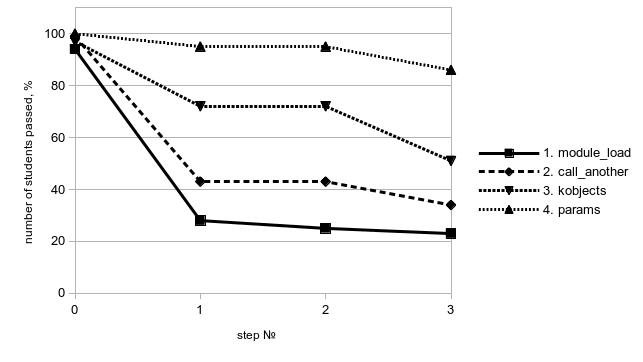
\includegraphics[width=\textwidth]{steps.jpg}
	\caption{Распределение студентов}
	\label{fig:mesh4}
\end{figure}

\section{Заключение}

\begin{thebibliography}{9}	
	\bibitem{likelytostop}
	{Taylor}, C. and {Veeramachaneni}, K. and {O'Reilly}, U.-M.
	\textit{Likely to stop? Predicting Stopout in Massive Open Online Courses}.
	ArXiv e-prints, 2014.
\end{thebibliography}

\end{document} % Конец текста.